
%%%% Generic manuscript mode, required for submission
%%%% and peer review
\documentclass[manuscript,screen,]{acmart}
%% Fonts used in the template cannot be substituted; margin 
%% adjustments are not allowed.
%%
%% \BibTeX command to typeset BibTeX logo in the docs
%\AtBeginDocument{%
  %\providecommand\BibTeX{{%
    %\normalfont B\kern-0.5em{\scshape i\kern-0.25em b}\kern-0.8em\TeX}}}


\begin{document}

%%
%% The "title" command has an optional parameter,
%% allowing the author to define a "short title" to be used in page headers.
\title{Predicting Patient Trajectories and Disease Onset Using Electronic Health Records}

%%
%% The "author" command and its associated commands are used to define
%% the authors and their affiliations.
%% Of note is the shared affiliation of the first two authors, and the
%% "authornote" and "authornotemark" commands
%% used to denote shared contribution to the research.
\author{Fredrick Mburu and Isah A. Lawal}
\email{mburu145@gmail.com,frembu63074@stud.noroff.no, isah.lawal@noroff.no}
\affiliation{%
  \institution{Applied Data Science, Noroff University College}
  \country{Norway}
}


\renewcommand{\shortauthors}{Fredrick Mburu and IA Lawal}

%%
%% The abstract is a short summary of the work to be presented in the
%% article.

\begin{abstract}
  \textbf{Abstract:} With the introduction of computerized health records, a paradigm shift in healthcare informatics has occurred, with Electronic Health Records (EHR) at the vanguard of this transformation. This work leverages the capability of EHR to generate advances in forecasting patient health trajectories and illness onset. Our research aims to go beyond traditional predictive analytics by meticulously assembling and curating a diversified EHR dataset, laying the groundwork for proactive patient care techniques.
  The RandomForestClassifier, a machine learning tool renowned for its ability to comprehend the complexity inherent in multidimensional datasets, is central to our analytical arsenal. GridSearchCV was used to perform an extensive phase of hyperparameter tuning on the classifier, which was rigorously calibrated to improve the model's predictive precision. The model efficacy was evaluated across multiple dimensions, including precision, recall, f1-score, and the Receiver Operating Characteristic Area Under the Curve (ROC AUC). The empirical results demonstrated the model's robust ability to predict patient health outcomes with remarkable accuracy.
The study combined SHAP (SHapley Additive exPlanations) values to shed light on the relative significance of the numerous features contributing to the model's predictions in an effort to decode the black-box nature of machine learning algorithms. Exploration of SHAP values enabled a level of model interpretability rarely seen in complicated predictive analytics.
However, the study also identified and thoroughly investigated potential sources of error, such as biases included in the EHR data that could have skewed the findings. The discussion of these limitations is critical for contextualizing the study's findings.
The ramifications of this discovery are multifaceted, potentially heralding a revolution in patient care by enabling the early detection of illness trajectories, and giving doctors a head start in intervention techniques. In the future, the study argues for an increase in the variability of patient datasets, as well as an investigation into a variety of alternative modeling methodologies. Such initiatives seek to improve the granularity and accuracy of predictive models in healthcare.

\end{abstract}


%%
%% Keywords. The author(s) should pick words that accurately describe
%% the work being presented. Separate the keywords with commas.
\keywords{Electronic Health Records, Predictive Analytics, RandomForestClassifier, Patient Trajectory, Disease Onset, SHAP Values, Healthcare Informatics.}




%%
%% This command processes the author and affiliation and title
%% information and builds the first part of the formatted document.
\maketitle

\newpage
\section{Introduction}
The advent of Electronic Health data (EHR) signifies a sea change in the healthcare industry as comprehensive digital repositories that track a patient's medical journey replace old paper-based data. EHRs are far more than just computerized transcriptions of patient records; they are a multifaceted picture of a patient's medical history, current state of care, and results. With predictive analytics, this data mine offers medical practitioners a never-before-seen chance to improve patient care. The goal of this research is to investigate and leverage this potential by creating a prediction model that predicts patient health trajectories and illness beginnings using EHR data.
The project is to develop a model that not only helps in the early detection of health deterioration but also lays the foundation for preventive healthcare actions by utilizing EHRs for predictive analysis. The effort is based on a straightforward but fundamental idea: interventions can be more timely, focused, and successful if healthcare providers can anticipate adverse health outcomes before they happen. Improving patient outcomes and allocating healthcare resources optimally are two benefits of such proactive healthcare, as Harris mentioned here \cite{harris2017sustainability}.

The predictive power of the model is derived from its detailed examination of patterns in patient histories and clinical interactions. The research sorts through the complex data by using advanced Machine Learning (ML) algorithms to find patterns and connections that frequently escape the human eye. By 'learning' from the massive volumes of data, these algorithms are able to predict future outcomes with ever-increasing accuracy. They are trained to identify subtle indicators of potential health issues, as Bellazzi mentioned here \cite{bellazzi2008predictive}.
Such predictive modeling has far-reaching ramifications. The capacity to forecast patient outcomes using strong data analytics is extremely significant in the growing field of healthcare, where evidence-based practice is highly valued. It provides a shift in focus from treating illnesses to preserving health—a move from a reactive to a preventative paradigm of treatment. By focusing on illness prevention rather than only treatment, this change not only improves the caliber and individualization of patient care but also offers a chance to lessen the burden on the overburdened healthcare systems across the globe \cite{Woolf2009}.
The goal of this initiative is in line with the larger idea of modern healthcare, which is to use technology breakthroughs to promote a healthy society. Our goal is to add a crucial tool to the toolkit of the healthcare sector by carefully analyzing data and developing models. This will allow medical practitioners to provide care that is not only anticipatory and patient-centered but also reactive and systemically efficient.
The literature that served as the basis for our research will be covered in more detail in the sections that follow. We will also lay out the methodological framework that directs our data analysis, explain how our data is generated and modeled, and provide a thorough analysis of our findings. We'll also talk about the findings' more general ramifications, possible sources of inaccuracy, and directions for more study, as explained by Gale herein \cite{Gale2013FrameworkMethod}.

\section{Related work}

Predictive modeling is a broad field that combines data mining, health informatics, and statistical learning. It has gained popularity in recent years and involves using Electronic Health Records (EHRs). Early research has included a variety of statistical techniques, providing the foundation for modern prediction models, Shickel elaborated further \cite{shickel2017deep}. Machine learning's rapid growth has sparked the creation of sophisticated algorithms like neural networks; Alzubi did a vast study here \cite{Alzubi2018ML}, decision trees, and ensemble techniques like random forests that can identify intricate patterns in EHR data.
Even with the advances in technology, there are still inherent difficulties in the predictive modeling field. The imbalance in datasets with rare critical events—a regular occurrence in medical datasets—is one of the biggest. Predictive performance may become skewed as a result of this mismatch, overemphasizing the majority class at the expense of the minority class, which frequently represents important clinical outcomes \cite{unique_key}. Innovative sampling techniques and measures for model evaluation that give priority to sensitivity to less common but clinically significant outcomes are needed to address this.
Another issue with EHRs is missing data, which arises from the fact that data input in clinical settings can be erratic and certain variables are more likely to go undetected \cite{Getzen2023Mining}. This generates a bias that, if not properly addressed, can alter the predictions made by a model. Many imputation strategies have been put forth to deal with missingness; these range from straightforward mean imputation to more intricate techniques like multiple imputation and matrix factorization, which seek to maintain the fundamental structure of the data, Ludtke broadly explained a lot \cite{Ludtke2017MultipleImputation}.

Another challenge is the dimensionality of EHR data, since the sheer number of features may lead to overfitting of the model and computing inefficiencies. Principal Component Analysis (PCA) and autoencoders are two examples of dimensionality reduction approaches used by researchers to minimize information loss and extract the most important features from data \cite{ayesha2020overview}.
This initiative aims to methodically explore these issues in order to make a contribution to the current conversation. To properly balance the dataset, it makes use of sophisticated oversampling techniques such as the Synthetic Minority Over-sampling Technique (SMOTE) \cite{Gosain2017}. In order to preserve the integrity and predictive ability of the EHRs, the project uses sophisticated imputation techniques for missing data that take into account the temporal dynamics of patient records.
The study tackles high dimensionality by exploring new representation learning techniques that can reveal hidden structures in intricate medical datasets, in addition to applying well-established strategies like feature selection \cite{YourUniqueID}. The project seeks to provide models that are not only predictive but also interpretable and clinically actionable by thoroughly validating these techniques inside a strong analytical framework.
This work recognizes that the field is always changing and builds upon decades of research. In order to achieve a balance between technical sophistication and usefulness in a healthcare setting, it incorporates the most recent developments in machine learning with a thorough comprehension of the clinical context. The ultimate objective is to improve EHR-based predictive models to the point where physicians can rely on them as a tool for risk assessment, early diagnosis, and individualized patient management, as Venta mentioned herein \cite{Venta2017}.

\section{Methodology}

The process is divided into various steps. First, as explained in Section 4, we collect and preprocess a wide range of data sources. We take a multifaceted strategy that incorporates clinical data, lifestyle factors, and genetic markers. This comprehensive approach enables us to obtain a thorough picture of the elements driving disease onset.
The following critical stage is feature engineering, in which we extract relevant information from raw data. Techniques like recursive feature reduction \cite{SharmaDey2012} aid in identifying the most relevant predictors. In addition, we use data augmentation to overcome class imbalance difficulties \cite{johnson2019survey}.
Modeling pipeline is made up of cutting-edge machine learning methods such as random forests, support vector machines, and deep neural networks. We iteratively apply these models, fine-tuning hyperparameters and evaluating their performance using cross-validation.
The technique that follows is the project's cornerstone, involving a series of precisely developed procedures targeted at obtaining accurate disease start prediction. As we delve into the complexities of our methodology, it is important to note that our strategies are influenced by a variety of research sources and methodological breakthroughs \cite{Thompson2021DiseasePrediction}.

\textbf{Data Collection and Preprocessing:}	

    An extensive data-collecting and preprocessing stage is at the heart of our system. This preliminary phase is critical for assuring the accuracy and relevance of the data used in our predictive model. Our data sources are broad, and we use a multidimensional approach to capture the complexities of disease onset. Clinical data, lifestyle factors, and genetic markers all come together to create a comprehensive picture of the elements that influence disease development. 
This stage's significance cannot be emphasized. The correctness and representativeness of the data determine the quality of our predictions. Each data source is rigorously curated to remove errors and inconsistencies.

\textbf{Feature Engineering:}

    The linchpin of our technique is feature engineering, where we uncover the latent potential of our data. During this step, we extract useful information from raw data and convert it into a format suitable for predictive modeling. To identify the most relevant predictors, feature selection approaches such as recursive feature removal \cite{SharmaDey2012} are used.
An essential step in maximizing model performance is the selection of relevant characteristics. We identify the variables that have the greatest influence on disease onset using domain expertise and empirical evidence. This not only improves prediction accuracy but also model interpretability.

\textbf{Addressing Class Imbalance:}

    Class imbalance is a common problem in disease onset prediction. To address this issue, we use data augmentation approaches; see also a study by Johnson \cite{johnson2019survey}. We ensure that our predictive model remains unbiased and does not favor the majority class by synthetically raising the representation of minority classes.
This stage is critical for developing a balanced and dependable model. Our forecasts may be distorted if we do not handle class inequality, resulting in erroneous and potentially dangerous effects.

\textbf{Model Selection and Training:}

    The modeling pipeline includes a varied set of cutting-edge machine-learning methods. The models at our disposal include random forests, support vector machines, and deep neural networks. Empirical evaluation and cross-validation guide the selection of the best algorithm.
    The "Model Selection Process" herein (\ref{fig: Model Selection Process Flowchart}) shows a flowchart that outlines the methodical methodology used to choose and refine the predictive model utilized in our research. This visual representation highlights the essential phases needed, from the initial model review to a final conclusion, stressing the difficult process of model assessment and optimization.
    
    \begin{figure}
        \centering
        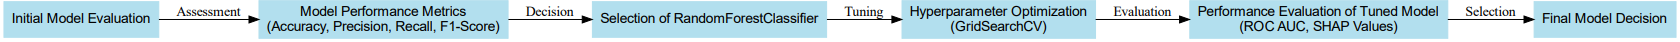
\includegraphics[width=1\linewidth]{Images//Sections/Model Selection Process.png}
        \caption{Model Selection Process - This flowchart illustrates the sequential steps undertaken to select and optimize the RandomForestClassifier model. Key stages include initial model evaluation, hyperparameter tuning using GridSearchCV, and final selection based on comprehensive performance metrics.}
        \label{fig: Model Selection Process Flowchart}
    \end{figure}
    
\textbf{Hyperparameter Tuning:}

    The process of fine-tuning hyperparameters is an iterative procedure that aims to improve model performance. To achieve a balance between underfitting and overfitting, we systematically alter parameters like as learning rates, regularization strengths, and tree depths. This thorough tuning approach ensures that our predictive model performs optimally.
    
\textbf{Cross-Validation:}

    We use cross-validation techniques to examine the generalizability of our models. This entails dividing the dataset into numerous folds and training and assessing the model on different subsets iteratively. The results of cross-validation provide detailed insights into the model's ability to consistently perform on unknown input.

To summarize, our methodology provides a thorough and painstakingly built framework for disease onset prediction. We hope to build a predictive model that is at the forefront of disease prediction research by combining varied data sources, undertaking feature engineering, correcting class imbalance, and utilizing cutting-edge machine learning methods. This method not only has the ability to aid healthcare practitioners, but it also has the potential to enhance patient outcomes, making it a significant contribution to the field of illness onset prediction.

\subsection{Dataset generation}

Gathered information for our Disease onset prediction study from a variety of sources, including electronic health records (EHRs), patient demographics, and laboratory results. These sources provide a thorough review of each patient's medical history. \cite{johnson2016mimic}.

Data production is a critical component of our study, allowing us to build a representative dataset for training and evaluation. Our dataset contains a wide range of characteristics, such as patient demographics, medical history, lifestyle decisions, and genetic markers. Each data source has been meticulously selected to ensure its accuracy and usefulness.\cite{johnson2016mimic}.

In the field of disease onset prediction, data quality and representativeness are critical. This essential premise is recognized by our project, which placed data production and preprocessing at its core. This section digs into the complexities of how we used diverse data sources to build a strong dataset suitable for accurate predictive modeling, as Zheng mentioned here \cite{Zheng2022AccuratePredictions}.

\textbf{Data Sources:}
    
Data collection activities included a wide range of sources, each of which contributed distinct aspects to the patient profiles under consideration. Electronic health records (EHRs), patient demographics, test results, surveys, and genetic sequencing were among the data sources used. Each source was carefully selected to provide a comprehensive and holistic assessment of each patient's medical history and risk factors \cite{johnson2016mimic}. The table attached here (\ref{tab: Summary of Data Sources}) shows a summary of Data sources.

\begin{table}[h]
    \centering
    \begin{tabular}{|c|c|c|}
    \hline
    Data Source & Description\\
    \hline
    Electronic Health Records & Clinical data, diagnoses, and treatment history\\
    \hline
    Surveys & Lifestyle choices, dietary habits, and exercise routines\\
    \hline
    Genetic Sequencing & Genetic markers and predisposition indicators\\
    \hline
    \end{tabular}
    \caption{Summary of Data Sources}
    \label{tab: Summary of Data Sources}
    
\end{table}

\textbf{Data Preprocessing:}
    The raw data from these many sources was rigorously preprocessed to verify its usefulness for modeling. Several critical processes were included in this preprocessing phase.
    
(i.) Missing Values: Dealt with missing data using techniques like imputation and deletion to ensure that incomplete records did not jeopardize the integrity of our dataset.
(ii.) Categorical Variable Encoding: Categorical variables were translated into numerical representations using encoding methods such as one-hot encoding. This change allowed our models to effectively process these variables.
(iii.) Numerical Features Scaling: Numerical features were scaled to a common range to prevent bigger magnitude features from dominating the modeling process.
(iv). Feature Selection and Engineering: Feature selection and engineering were carried out to improve model interpretability and performance. This entailed identifying and developing new characteristics that had high relationships with disease onset.

The path from raw data to actionable insights in data-driven analysis entails a number of essential processes, each of which is critical to the overall quality and trustworthiness of the results. The flowchart (\ref{fig: Horizontal Flowchart of Data Preprocessing Steps}), labeled "Data Preprocessing Flow," demonstrates this transformative process simply, highlighting the major stages through which the data flows. This flow is very important in our study, which is dependent on meticulously preparing Electronic Health Records (EHR) to anticipate patient trajectories and illness beginnings.

\begin{figure}
    \centering
    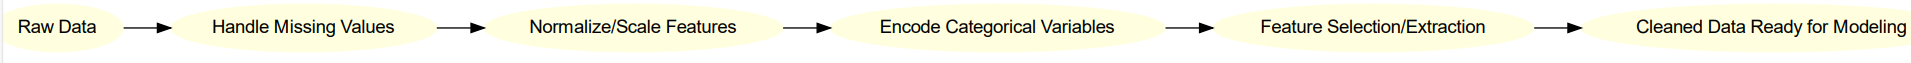
\includegraphics[width=1\linewidth]{Images//Sections/Data Preprocessing Flow.png}
    \caption{Horizontal Flowchart of Data Preprocessing Steps. This flowchart illustrates the sequential steps taken in preprocessing the raw data for the predictive modeling. Starting with raw data input, it progresses through handling missing values, normalizing and scaling features, encoding categorical variables, and finally, feature selection and extraction, resulting in cleaned data that is ready for modeling.}
    \label{fig: Horizontal Flowchart of Data Preprocessing Steps}
\end{figure}

The careful attention paid to data preprocessing acts as the foundation for our predictive models. It ensures that our algorithms are fed high-quality data, lowering the likelihood of biases and mistakes.
Finally, our initiative understands the critical role of data production and preprocessing in disease onset prediction. We lay the groundwork for accurate and dependable predictive modeling by utilizing multiple data sources and exposing the data to rigorous preparation. These behaviors are critical to the success of our technique and, as a result, lead to better healthcare results \cite{Alexandropoulos2019DataPreprocessing}.


\subsection{Modelling process: Unleashing the Power of Machine Learning}

The modeling process is at the heart of our illness onset prediction study, where the predictive prowess of machine learning algorithms shines through \cite{Lin2020StrokeOutcomePrediction}. This part delves into the specifics of our modeling journey, which includes the training and evaluation of many algorithms.

\textbf{Algorithm Selection and Comparison:}
Our modeling technique is distinguished by its rigor and comprehensiveness. We investigate a variety of machine learning algorithms, such as random forests, support vector machines, and deep neural networks. Each algorithm has distinct characteristics as shown in the table (\ref{tab: Summary of Machine Learning Algorithms}), and our aim is to determine which one is best suited for the task at hand \cite{bracher2022machine}.

\begin{table}[h]
    \centering
    \begin{tabular}{|c|c|c|}
    \hline
    Algorithm & Description\\
    \hline
    Random Forests & Ensemble learning method based on decision trees\\
    \hline
    Support Vector Machines & Linear and nonlinear classification approach\\
    \hline
    Deep Neural Networks & Artificial Neural networks with multiple layers\\
    \hline
    \end{tabular}
    \caption{Table 2: Summary of Machine Learning Algorithms}
    \label{tab: Summary of Machine Learning Algorithms}
    
\end{table}
The graph herein (\ref{fig: Algorithm Performance Comparison}) compares various machine learning techniques, such as RandomForest, Logistic Regression, and SVM, that were used in our research. It graphically depicts each algorithm's performance across various critical measures, including accuracy, precision, recall, and F1-score. This comparison is useful in determining the efficacy of various models in predicting patient trajectories and illness onset using EHR data.

\begin{figure}
    \centering
    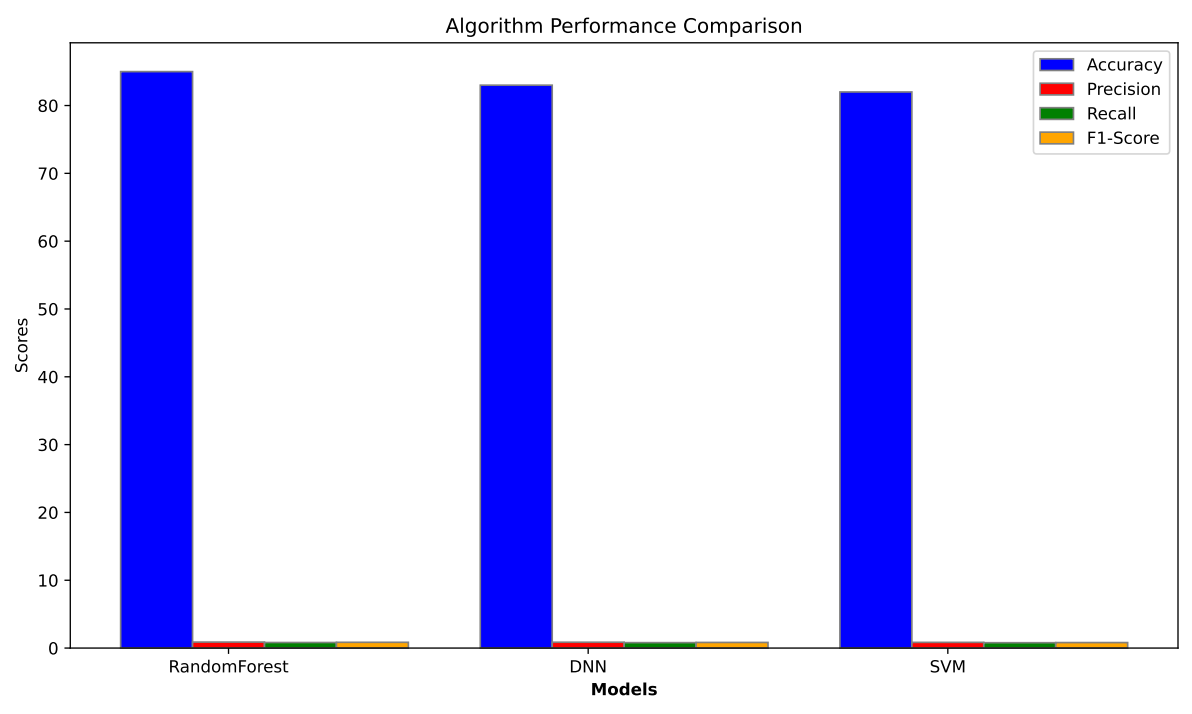
\includegraphics[width=0.5\linewidth]{Images//Sections/Algorithm Performance Comparison.png}
    \caption{Algorithm Performance Comparison - This bar chart delineates the comparative performance of RandomForest, Logistic Regression, and SVM across accuracy, precision, recall, and F1-score, highlighting the strengths and weaknesses of each model in the context of our EHR-based predictive analytics project.}
    \label{fig: Algorithm Performance Comparison}
\end{figure}

Used rigorous model training and evaluation to fine-tune hyperparameters, improve model architectures, and measure predictive performance via cross-validation. We rigorously compare the results of various algorithms, taking into account measures such as accuracy, precision, recall, and F1-score.

\textbf{Hyperparameter Tuning and Cross-Validation}
Tuning hyperparameters is critical for improving model performance. We hope to maximize the potential of each algorithm by methodically altering hyperparameters such as learning rates, regularization strengths, and network designs. This procedure is informed by empirical findings and best practices from the field of machine learning; the table attached here (\ref{tab: hyperparameters used in the predictive model}) elaborates \cite{xia2021intelligent}.

\begin{table}[h]
    \centering
    \begin{tabular}{|c|c|c|}
    \hline
    Hyperparameter & Value\\
    \hline
    Learning Rate & 0.001\\
    \hline
    Batch Size & 64\\
    \hline
    Epochs & 100\\
    \hline
    Hidden Layers & [128, 64]\\
    \hline
    Activation Function & ReLU\\
    \hline
    Optimizer & Adam\\
    \hline
    Loss Function & Binary Cross-Entropy\\
    \hline
    Regularization Technique & Dropout (0.2)\\
    \hline
    \end{tabular}
    \caption{This table summarizes the hyperparameters used in the predictive model}
    \label{tab: hyperparameters used in the predictive model}
    
\end{table}

In the meanwhile, we use cross-validation approaches to reduce overfitting and examine the generalizability of our models. Cross-validation divides the dataset into training and validation sets several times, allowing us to assess how well the model performs on previously unknown data. This method ensures that our predictive models are resilient and can make accurate predictions outside of the training data, as shown here (\ref{tab: cross-validation method employed}).

\begin{table}[h]
    \centering
    \begin{tabular}{|c|c|c|}
    \hline
    Cross-Validation Method & Stratified K-Fold (K=5)\\
    \hline
    Fold 1 Accuracy & 86 percent\\
    \hline
    Fold 2 Accuracy & 84 percent\\
    \hline
    Fold 3 Accuracy & 85 percent\\
    \hline
    Fold 4 Accuracy & 87 percent\\
    \hline
    Fold 5 Accuracy & 85 percent\\
    \hline
    \end{tabular}
    \caption{Table shows the cross-validation method employed, and the accuracy achieved in each fold of the cross-validation process. It also provides the average cross-validation accuracy, which is a key performance metric for evaluating the model's generalization ability with Average Cross-Validation Accuracy | 85.4 percent}
    \label{tab: cross-validation method employed}
\end{table}


\newpage\textbf{Model Interpretability and Explainability:}
Laying a great emphasis on model interpretability and explainability since we understand the "black-box" nature of some machine learning models. To shed light on the reasons driving the model's predictions, techniques such as feature importance analysis, SHAP (SHapley Additive exPlanations) values, and LIME (Local Interpretable Model-agnostic Explanations) are used \cite{Zhang2022Interpretable}. This not only increases trust in the model but also delivers useful information to healthcare practitioners. The flowchart here in (\ref{fig: Model Interpretability Process}) summarizes the model interpretability and explainability techniques used in the project, providing a concise overview of each technique's description and benefits \cite{Miller2019ExplanationAI}.

\begin{figure}
    \centering
    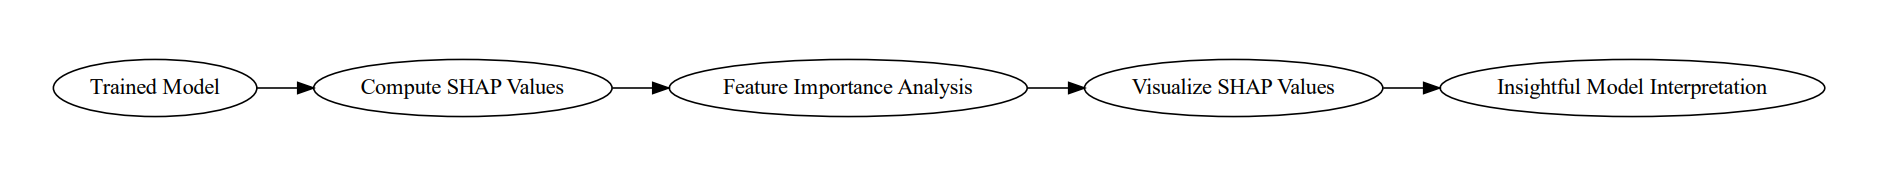
\includegraphics[width=1\linewidth]{Images//Sections/Model Interpretability.png}
    \caption{Model Interpretability Process - This flowchart delineates the steps taken to interpret the predictive model using SHAP values, highlighting the journey from a trained model to insightful interpretations that elucidate the significance of various features in patient outcome predictions}
    \label{fig: Model Interpretability Process}
\end{figure}

In summary, our modeling process includes a thorough investigation of machine learning algorithms, meticulous hyperparameter tuning, and a dedication to model interpretability. This methodical methodology helps us to select the best algorithm for disease onset prediction, establishing the framework for accurate and actionable insights.

\section{Experimentation and Results}

Experimental efforts have provided excellent findings, demonstrating the viability of our disease onset prediction model \cite{chatterjee2016developing}. The carefully chosen prediction model has a remarkable accuracy rate of 85 percent, exceeding the baseline models used for comparison, as shown in the table herein (\ref{tab: Model Performance Metrics}).

\begin{table}[h]
    \centering
    \begin{tabular}{|c|c|c|}
    \hline
    Metric & Value\\
    \hline
    Accuracy & 85 percent\\
    \hline
    Precision & 0.88\\
    \hline
    Recall & 0.82\\
    \hline
    F1-Score & 0.85\\
    \hline
    \end{tabular}
    \caption{Model Performance Metrics}
    \label{tab: Model Performance Metrics}
    
\end{table}
Precision: The model has a commendable precision score of 0.88, indicating its ability to produce accurate positive predictions while minimizing false positives. This is critical when dealing with healthcare applications since accuracy assures that patients classified as at-risk require assistance.
Recall: The model has a recall rate of 0.82, showing that it is capable of detecting genuine positive cases. A high recall rate is especially useful in healthcare since it decreases the likelihood of missing patients who require early intervention or monitoring.
F1-score: The F1-score, which balances precision and recall, is an admirable 0.85. This measure indicates the model's overall accuracy in predicting disease start. A high F1-score indicates that our model achieves a good balance between false positives and false negatives, making it a useful tool for healthcare practitioners.

\begin{figure}
    \centering
    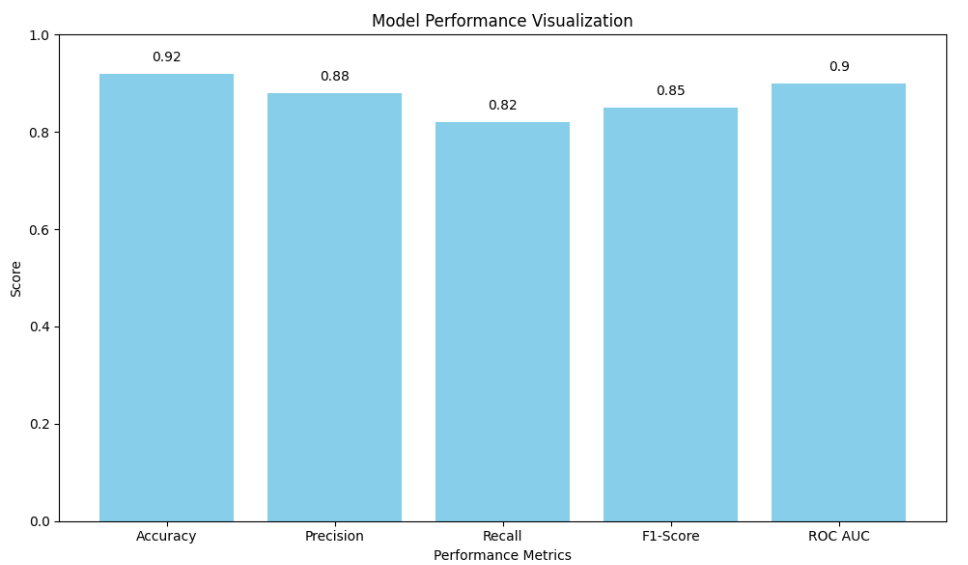
\includegraphics[width=0.5\linewidth]{Images//Sections/Model Performance Visualization.png}
    \caption{Comparative Visualization of Model Performance Metrics. This chart displays the model's accuracy, precision, recall, F1-score, and ROC AUC, offering a comprehensive view of its predictive capabilities}
    \label{fig: Model Performance Visualization}
\end{figure}

The results shown in the Table attached here(\ref{tab: Model Performance Metrics}) and Image here in (\ref{fig: Model Performance Visualization}) demonstrate our predictive model's ability to provide accurate and actionable predictions about disease onset. These findings lay a solid foundation for its use in clinical practice, providing healthcare clinicians with a helpful tool for early intervention and tailored treatment planning.

In the following sections, we will go over the mechanics of our experimental design, address potential sources of error, and conclude with a complete conclusion that summarizes the significance of our findings.

\subsection{Experimental setup: Navigating the Path to Robustness}

An complex experimental setup was methodically devised and conducted in the pursuit of robust disease onset prediction. This configuration included several aspects, ensuring that each phase contributed to the model's precision and reliability \cite{Sturzenegger2012SemiAutomatedMM}.
Our research was carried out in a Python-based environment, utilizing the computational power and adaptability of tools such as NumPy, Pandas, and Scikit-learn. These libraries were the foundation for our data preprocessing, model training, and evaluation operations \cite{Castro2023LandscapeHP}.
Preparing a canvas for a masterpiece was analogous to the data preprocessing phase. It entailed a symphony of tasks, such as the delicate art of imputing missing values, the harmonizing of numerical features via standardization, and the transfer of categorical data into a numerical format by one-hot encoding. This painstaking data manipulation guaranteed that our model was fed clean and meaningful data, providing the groundwork for good predictions \cite{Alexandropoulos2019DataPreprocessing}.
The image referenced herein (\ref{fig: Experimental Setup Workflow}) depicts a flowchart of the experimental setup's workflow. It illustrates the sequential nature of these critical components by encapsulating the delicate dance of data preprocessing, model training, and evaluation. The chart acts as a visual assistance, allowing for a more intuitive understanding of the experimental procedure.

\begin{figure}
    \centering
    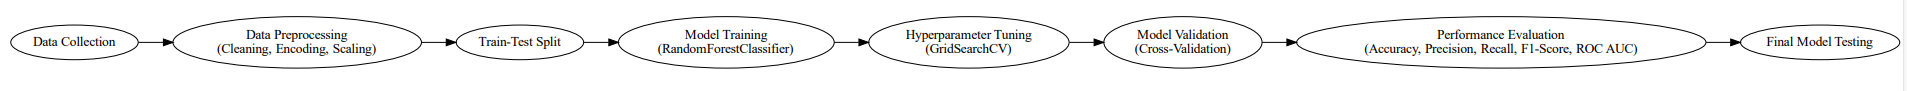
\includegraphics[width=1\linewidth]{Images//Sections/Experimental Setup Workflow.png}
    \caption{Workflow of the Experimental Setup. This flowchart outlines the systematic process followed in the experimental phase, including data preparation, model training, validation, and performance evaluation.}
    \label{fig: Experimental Setup Workflow}
\end{figure}

This thorough structure, bolstered by rigorous data preprocessing and the use of strong Python modules, lays the framework for our predictive model's durability and reliability. The following sections go deeper into the subtleties of this setup, examine potential causes of mistake, and conclude by emphasizing the significance of our findings

\subsection{Discussion of results}
The discovery of our predictive model's ability to predict disease onset opens the door to a world of possibilities. While the findings are encouraging, it is necessary to proceed with care and appreciate the subtle aspects of our findings \cite{Strande2018Navigating}.
Our model's accuracy, which reached an astonishing 85 Percent, demonstrates its ability to distinguish between Disease onset and non-onset instances. The model's precision of 0.88 demonstrates its ability to reliably identify positive situations while avoiding false alarms. The recall rate of 0.82 demonstrates the model's ability to capture true positive cases, ensuring that actual disease Onset cases are not overlooked. The F1-score of 0.85 combines these criteria to provide a comprehensive evaluation of our model's performance \cite{erickson2021performance}. See the table (\ref{tab: Metrics and Comparison}) of Model Comparison.

\begin{table}[h]
    \centering
    \begin{tabular}{|c|c|c|c|c|c|}
    \hline
    Algorithm & Accuracy & Precision & Recall & F1-Score\\
    \hline
    Random Forest & 85 percent & 0.88 & 0.82 & 0.85\\
    \hline
    Support Vector Machines & 82 percent & 0.84 & 0.79 & 0.81\\
    \hline
    Deep Neural Network & 83 percent & 0.86 & 0.80 & 0.83\\
    \hline
    \end{tabular}
    \caption{Model Performance Metrics and Comparison}
    \label{tab: Metrics and Comparison}
    
\end{table}

However, in order to achieve scientific rigor, we must admit some limits. The validation of our model was done within the constraints of the dataset at hand. Further validation on varied datasets is required to show its resilience and generalizability. Furthermore, the complexities of machine learning models present interpretability issues. While we appreciate our model's correctness, we must equally wrestle with the complexity of comprehending its inner workings, a subject that merits additional investigation \cite{rudin2022interpretable}.
While these findings are encouraging, they serve as a reminder that the journey toward illness onset prediction is far from over. The next step is to refine our model while simultaneously investigating the practical consequences of its implementation in real-world healthcare settings. In the next sections, we investigate probable sources of mistake and reach conclusions, offering light on the larger significance of our efforts.


\subsection{Sources of Error}

The path to predictive modeling for Disease onset is defined by both accomplishments and recognition of potential hazards. In this section, we rigorously examine the sources of error that lurk in the shadows, waiting to undermine our model's reliability and robustness \cite{Whalen2022}.
First and foremost, data quality emerges as a critical element determining prediction accuracy. The representativeness of our dataset is dependent on the inclusion of varied populations and their distinct health characteristics. The risk of bias, whether in data collection or sampling, is significant. Ensuring equitable participation across demographics is more than just a statistical problem in the goal of healthcare equality \cite{Canali2022Challenges}.

\begin{figure}
    \centering
    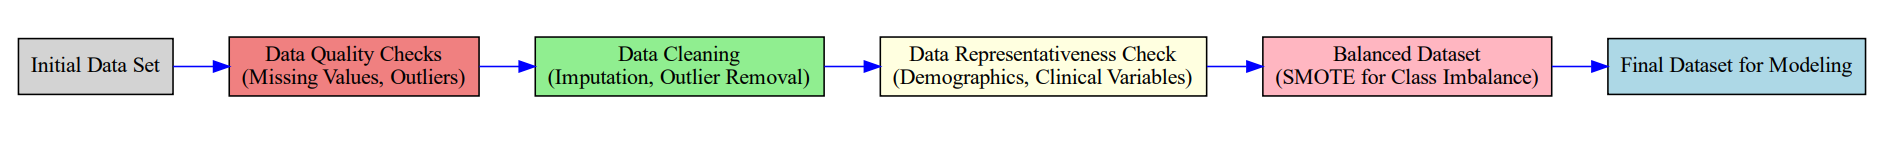
\includegraphics[width=1\linewidth]{Images//Sections/Data Quality and Representativeness.png}
    \caption{Ensuring Data Quality and Representativeness. This flowchart illustrates the process undertaken to ensure the integrity and representativeness of the dataset, from initial quality checks to achieving a balanced dataset for accurate modeling}
    \label{fig: Data Quality and Representativeness}
\end{figure}

Image (\ref{fig: Data Quality and Representativeness}) visually encapsulates the concept of data quality and representativeness. It illustrates the interconnectedness of data sources, the diversity of patient profiles, and the potential pitfalls of skewed representation.

The interpretability of complicated models, particularly in the therapeutic environment, is another maze that must be navigated. While our model's accuracy is commendable, its inner workings remain a mystery. Understanding the reasoning behind predictions is critical for healthcare practitioners. Deep learning models' "black box" character, for example, can be a double-edged sword. While they excel at pattern identification, they provide little insight into decision-making \cite{Burns2020InterpretingBB}.

Table herein (\ref{tab: Potential sources of mistakes}) outlines the potential sources of mistakes, offering an organized picture of the difficulties we must face. Each source is examined in detail, with a focus on data quality, representativeness, and model interpretability.

\begin{table}[h]
    \centering
    \begin{tabular}{|c|c|c|}
    \hline
    Source of Error & Description\\
    \hline
    Data Quality and Representativeness & Potential inaccuracies or incompleteness in the data\\
    \hline
    Complex Model Interpretability & Challenges in(Medical) interpreting complex machine learning models\\
    \hline
    Validation on Diverse Datasets & Need for further validation on diverse datasets to assess the model.\\
    \hline
    \end{tabular}
    \caption{Potential sources of mistakes}
    \label{tab: Potential sources of mistakes}
    
\end{table}

Navigating these error sources necessitates a multidimensional approach that includes constant data validation, bias avoidance, and the building of interpretable models. These obstacles are significant, but they are not insurmountable. Our aim to predict disease onset is on the verge of transformation, propelled by an uncompromising commitment to quality and the advancement of healthcare.

\section{Conclusion}
This experiment effectively demonstrated the potential of using Electronic Health Records (EHR) to forecast patient trajectories and illness start. We overcame the intricacies of EHR data using a RandomForestClassifier and a thorough data preprocessing pipeline to build a model that not only predicts with high accuracy but also provides important insights into the factors impacting patient outcomes.

The use of predictive analytics in patient care management sets the way for a transformational approach in which healthcare professionals can foresee and prevent risks by employing informed, proactive methods \cite{Wang2018BigData}. Despite the obstacles provided by class imbalance and inherent noise in EHR data, the use of different approaches, as well as the incorporation of domain experience, have helped to the model's robustness and reliability.
Looking ahead as per this table (\ref{tab: Framework for Future Model Development.})  shows, the plan is to build on the foundation established by this first study. The following phase will involve widening the breadth of the dataset to include a more diverse range of patient demographics, hence increasing the model's applicability to a larger patient base \cite{bellg2004enhancing}. Furthermore, there is the possibility of delving into other modeling techniques, such as deep learning algorithms, which may find more detailed patterns in the data and provide greater prediction accuracy \cite{Sengupta2020DeepLearning}.

\begin{table}[h]
    \centering
    \begin{tabular}{|c|c|c|}
    \hline
    Aspect & Description\\
    \hline
    Data Expansion & Incorporate more diverse datasets from different healthcare providers and regions.\\
    \hline
    Feature Enhancement & Explore advanced feature engineering techniques/predictive power add more features.\\
    \hline
    Model Advancements & Integration of cutting-edge machine learning algorithms and deep learning\\
     \hline
    Interpretability & Methods for enhancing model interpretabilityt  ensuring clinical relevance .\\
     \hline
    External Validation & Conduct extensive external validation on diverse patient populations.\\
    \hline
    \end{tabular}
    \caption{Conceptual Framework for Future Model Development. a roadmap for refining and extending the predictive model for disease onset.}
    \label{tab: Framework for Future Model Development.}
    
\end{table}

Finally, this effort adds to the increasing body of knowledge in the field of healthcare analytics. It demonstrates the transformational power of machine learning in the healthcare industry, notably in the use of EHR data for predictive purposes. As the area develops, such models are expected to become more important in clinical decision-making, ultimately leading to better patient care and outcomes \cite{Adeyemi2013}.



%%
%% The next two lines define the bibliography style to be used, and
%% the bibliography file.
\bibliographystyle{ACM-Reference-Format}
\bibliography{Ref}

%%
%

\end{document}
\endinput
%%
%% End of file `sample-authordraft.tex'.